
% ════════════════════════════════════════════
% 模型求解（5.4.4.模型求解.tex，三级子块）
% ════════════════════════════════════════════
\subsubsection{波动电价下的重算结果与对比}

本节用附件四的波动电价数据重新求解问题二与问题三，仍以 1 月为预热期、费用汇总仅统计 2 月 1 日—12 月 31 日。问题二沿用 0:00 预测、按 5 倍紧急电价制定计划购电、实际运行后滚动结算紧急购电的三段式框架：全年 334 天计划购电费 13895479.01 元、紧急购电 304292.65 kWh、紧急购电费 1181652.65 元，合计 15077131.66 元；问题三在该电价下的滚动优化总费用为 14956526.18 元。

波动电价下问题二（result4-2）与问题三（result4-3）的指定时段购电量、全天购电量与购电费列入表~\ref{tab:结果4-2}，储能充放电量见表~\ref{tab:结果4-2b}，四个指定日期的费用汇总见表~\ref{tab:结果4-1}。负载与光伏预测误差同样使四个指定日期出现计划外偏差，紧急购电时段分布与固定电价情形相近（表~\ref{tab:结果2-3}、表~\ref{tab:结果3-3}），差异主要来自计划购电随电价的小幅变化。四个典型日的全天购电量在问题三下均低于问题二。

{\footnotesize\renewcommand{\arraystretch}{0.95}\begin{longtable}{>{\centering\arraybackslash}p{0.07\textwidth}>{\centering\arraybackslash}p{0.19\textwidth}>{\centering\arraybackslash}p{0.16\textwidth}>{\centering\arraybackslash}p{0.16\textwidth}>{\centering\arraybackslash}p{0.16\textwidth}>{\centering\arraybackslash}p{0.16\textwidth}}
  
  \caption{2025 年四个典型日微网在指定时间段的购电量（kWh）及全天购电量（kWh）与购电费（元）；10:00--10:10 与 14:00--14:10 两个指定时段四日均未购电（0.00）}
  \label{tab:结果4-2} \\
  \toprule
  问题 & 项目 & 2025.3.20 & 2025.6.21 & 2025.9.23 & 2025.12.21 \\
  \midrule
  \endfirsthead
  \caption{2025 年四个典型日微网在指定时间段的购电量（kWh）及全天购电量（kWh）与购电费（元）（续）} \\
  \toprule
  问题 & 项目 & 2025.3.20 & 2025.6.21 & 2025.9.23 & 2025.12.21 \\
  \midrule
  \endhead
  \bottomrule
  \endfoot
  \multirow{9}{*}{问题二} & 12:00--12:10 & 535.11 & 0.00 & 528.89 & 954.41 \\
   & 16:00--16:10 & 506.24 & 159.03 & 561.39 & 844.76 \\
   & 18:00--18:10 & 0.00 & 225.46 & 0.00 & 742.25 \\
   & 20:00--20:10 & 0.00 & 0.00 & 845.29 & 0.00 \\
   & 全天购电量 & 68480.76 & 35093.50 & 71715.57 & 98238.82 \\
   & 全天购电费 & 42307.23 & 16867.61 & 45906.41 & 74152.25 \\
   & 全天紧急购电量 & 1506.23 & 424.89 & 707.03 & 875.82 \\
   & 全天紧急购电费 & 5386.82 & 1499.51 & 3131.71 & 3881.15 \\
   & 全天合计购电费 & 47694.05 & 18367.12 & 49038.12 & 78033.40 \\
  \cmidrule(lr){1-6}
  \multirow{6}{*}{问题三} & 12:00--12:10 & 560.43 & 0.00 & 371.59 & 979.54 \\
   & 16:00--16:10 & 663.99 & 111.20 & 636.70 & 799.69 \\
   & 18:00--18:10 & 0.00 & 0.00 & 0.00 & 715.41 \\
   & 20:00--20:10 & 0.00 & 0.00 & 827.18 & 0.00 \\
   & 全天购电量 & 67887.93 & 33099.44 & 68433.17 & 93474.87 \\
   & 全天购电费 & 41997.87 & 15620.14 & 44112.85 & 69824.09 \\
\end{longtable}}

{\footnotesize\renewcommand{\arraystretch}{0.95}\begin{longtable}{>{\centering\arraybackslash}p{0.12\textwidth}>{\centering\arraybackslash}p{0.18\textwidth}>{\centering\arraybackslash}p{0.165\textwidth}>{\centering\arraybackslash}p{0.165\textwidth}>{\centering\arraybackslash}p{0.165\textwidth}>{\centering\arraybackslash}p{0.165\textwidth}}
  
  \caption{2025 年四个典型日储能设备在指定时间段的充放电量（kWh），每格按“充电量/放电量”列出；四个典型日 0:00 与 24:00 的储电量均为 1200.00 kWh}
  \label{tab:结果4-2b} \\
  \toprule
  问题 & 时间段 & 2025.3.20 & 2025.6.21 & 2025.9.23 & 2025.12.21 \\
  \midrule
  \endfirsthead
  \caption{2025 年四个典型日储能设备在指定时间段的充放电量（kWh）（续）} \\
  \toprule
  问题 & 时间段 & 2025.3.20 & 2025.6.21 & 2025.9.23 & 2025.12.21 \\
  \midrule
  \endhead
  \bottomrule
  \endfoot
  \multirow{6}{*}{问题二} & 00:00--04:00 & 6666.67/0.00 & 1666.67/1350.00 & 5833.33/0.00 & 9000.00/0.00 \\
   & 04:00--08:00 & 4000.00/5829.15 & 2690.00/2155.42 & 4833.33/6060.24 & 1666.67/833.33 \\
   & 08:00--12:00 & 6050.98/2810.85 & 6251.06/0.00 & 5907.57/2579.76 & 5833.33/7806.67 \\
   & 12:00--16:00 & 5029.62/335.29 & 4386.62/0.00 & 4932.08/140.12 & 7500.00/2695.30 \\
   & 16:00--20:00 & 0.00/6416.42 & 0.00/6124.20 & 0.00/6973.33 & 660.87/5275.65 \\
   & 20:00--24:00 & 833.33/2898.58 & 756.82/3128.83 & 0.00/1666.67 & 0.00/3364.35 \\
  \cmidrule(lr){1-6}
  \multirow{6}{*}{问题三} & 00:00--04:00 & 6666.67/0.00 & 1666.67/1350.00 & 5833.33/0.00 & 9000.00/0.00 \\
   & 04:00--08:00 & 4000.00/6149.96 & 2242.74/1816.62 & 4833.33/6435.18 & 1666.67/835.79 \\
   & 08:00--12:00 & 4106.95/2313.92 & 1812.59/0.00 & 5130.10/1920.52 & 5833.33/7547.60 \\
   & 12:00--16:00 & 6651.73/250.65 & 8839.57/0.00 & 5575.59/315.91 & 7500.00/2432.26 \\
   & 16:00--20:00 & 0.00/6412.35 & 14.50/6154.10 & 0.00/7021.77 & 19.32/5171.86 \\
   & 20:00--24:00 & 833.33/2902.65 & 748.18/3091.92 & 0.00/1618.23 & 0.00/3468.14 \\
\end{longtable}}

\begin{table}[H]
  \centering
  \footnotesize
  \caption{波动电价下指定日期的问题三总费用与紧急购电费（元）；问题二全天合计购电费见表~\ref{tab:结果4-2}}
  \label{tab:结果4-1}
  \begin{tabular}{ccc}
  \toprule
  日期 & 问题三总费用 & 紧急购电费 \\
  \midrule
  2025.3.20 & 54192.97 & 13666.00 \\
  2025.6.21 & 17963.88 & 1618.00 \\
  2025.9.23 & 49152.77 & 5928.00 \\
  2025.12.21 & 75009.33 & 4147.00 \\
  \bottomrule
  \end{tabular}
\end{table}

四季典型日的购电功率对电价波动更为灵敏：夜间低电价时段购电与充电功率明显增大，白天高电价时段购电被压缩，低充高放套利更积极（图~\ref{fig:结果4-2}）。

\begin{figure}[H]
    \centering
    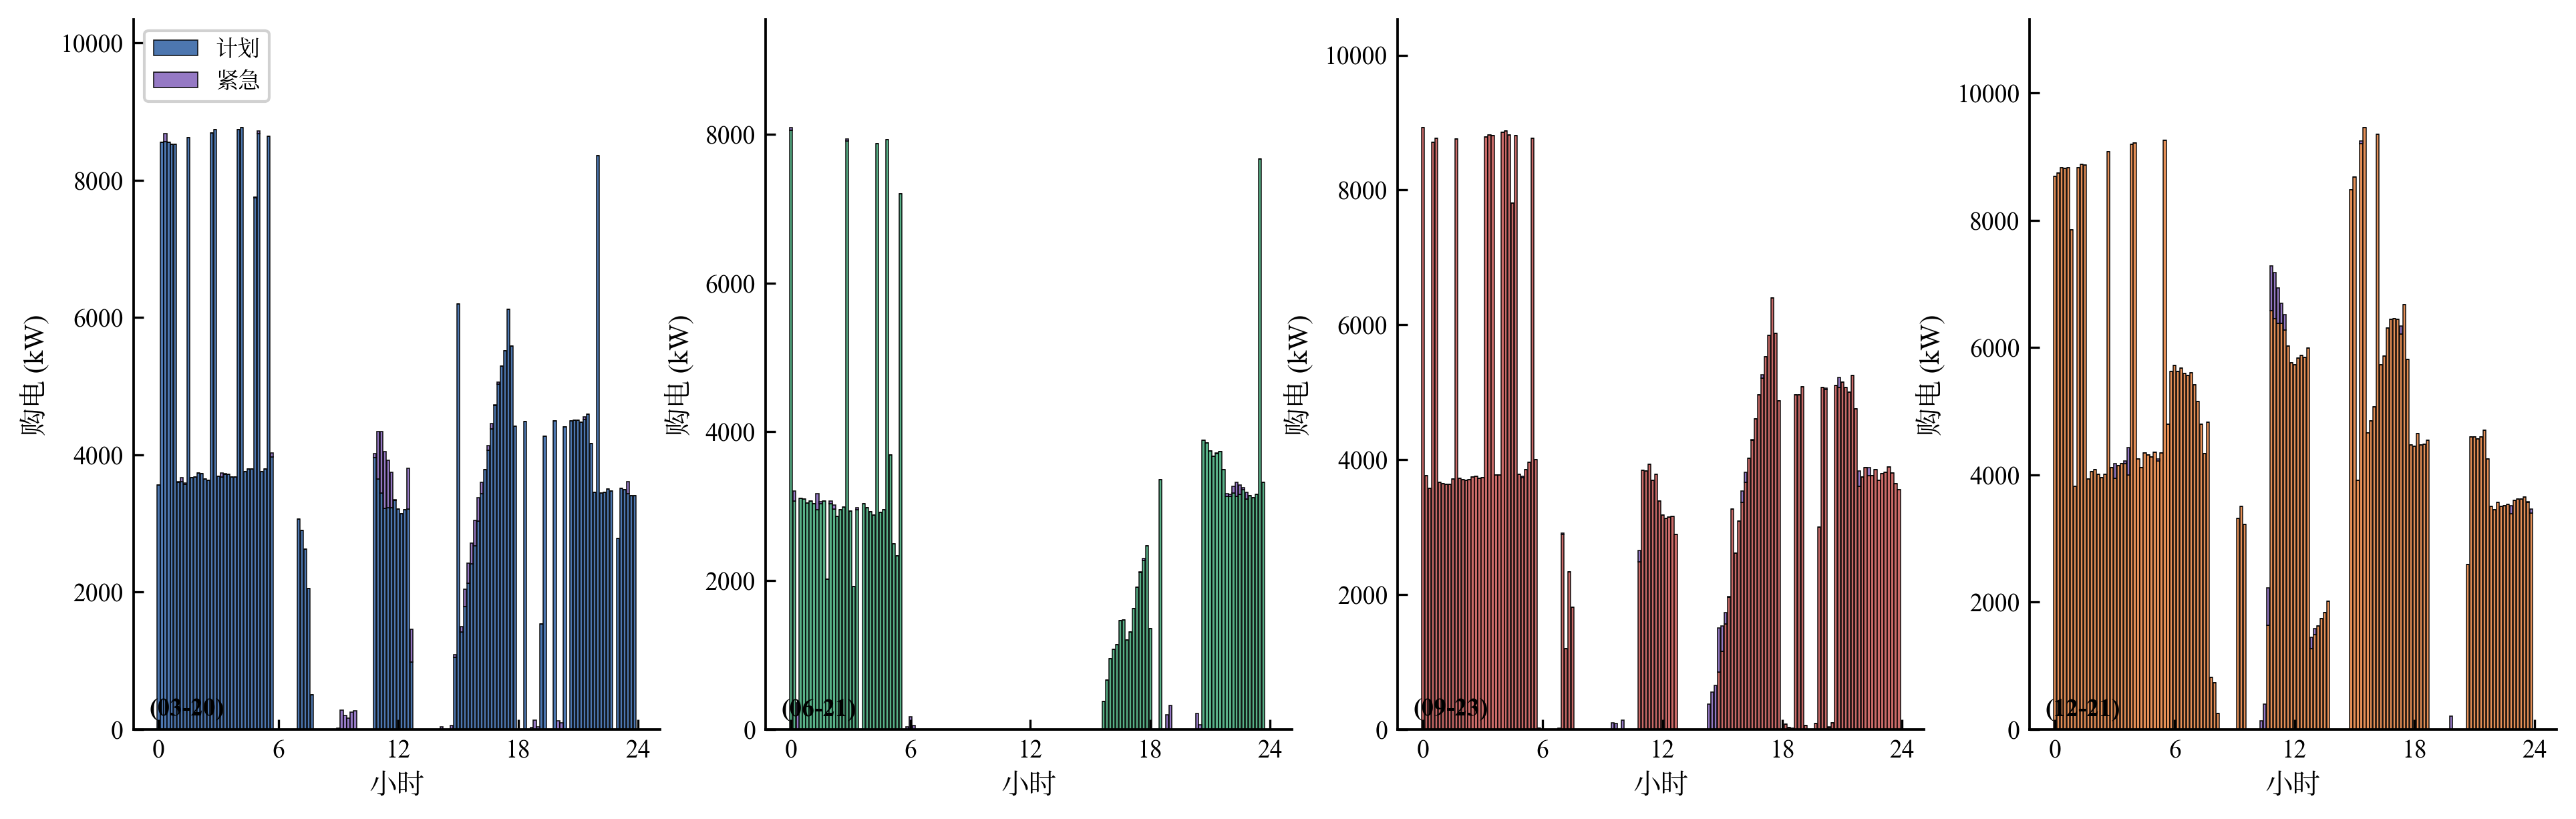
\includegraphics[width=0.42\textwidth]{求解/问题四/图片/图4-2_波动电价四季典型日购电.png}
    \caption{波动电价下四季典型日购电策略}
    \label{fig:结果4-2}
\end{figure}

光伏预报更新后，调整策略仍在预报时点修正购电功率，幅度因电价波动而异，方向仍以减小供电缺口、压缩高价时段购电为主；储能荷电状态日内多次充放切换以适应峰谷变化，全程满足容量约束，峰谷价差转化为套利收益（图~\ref{fig:结果4-3}）。

\begin{figure}[H]
    \centering
    \begin{minipage}[t]{0.44\textwidth}
        \centering
        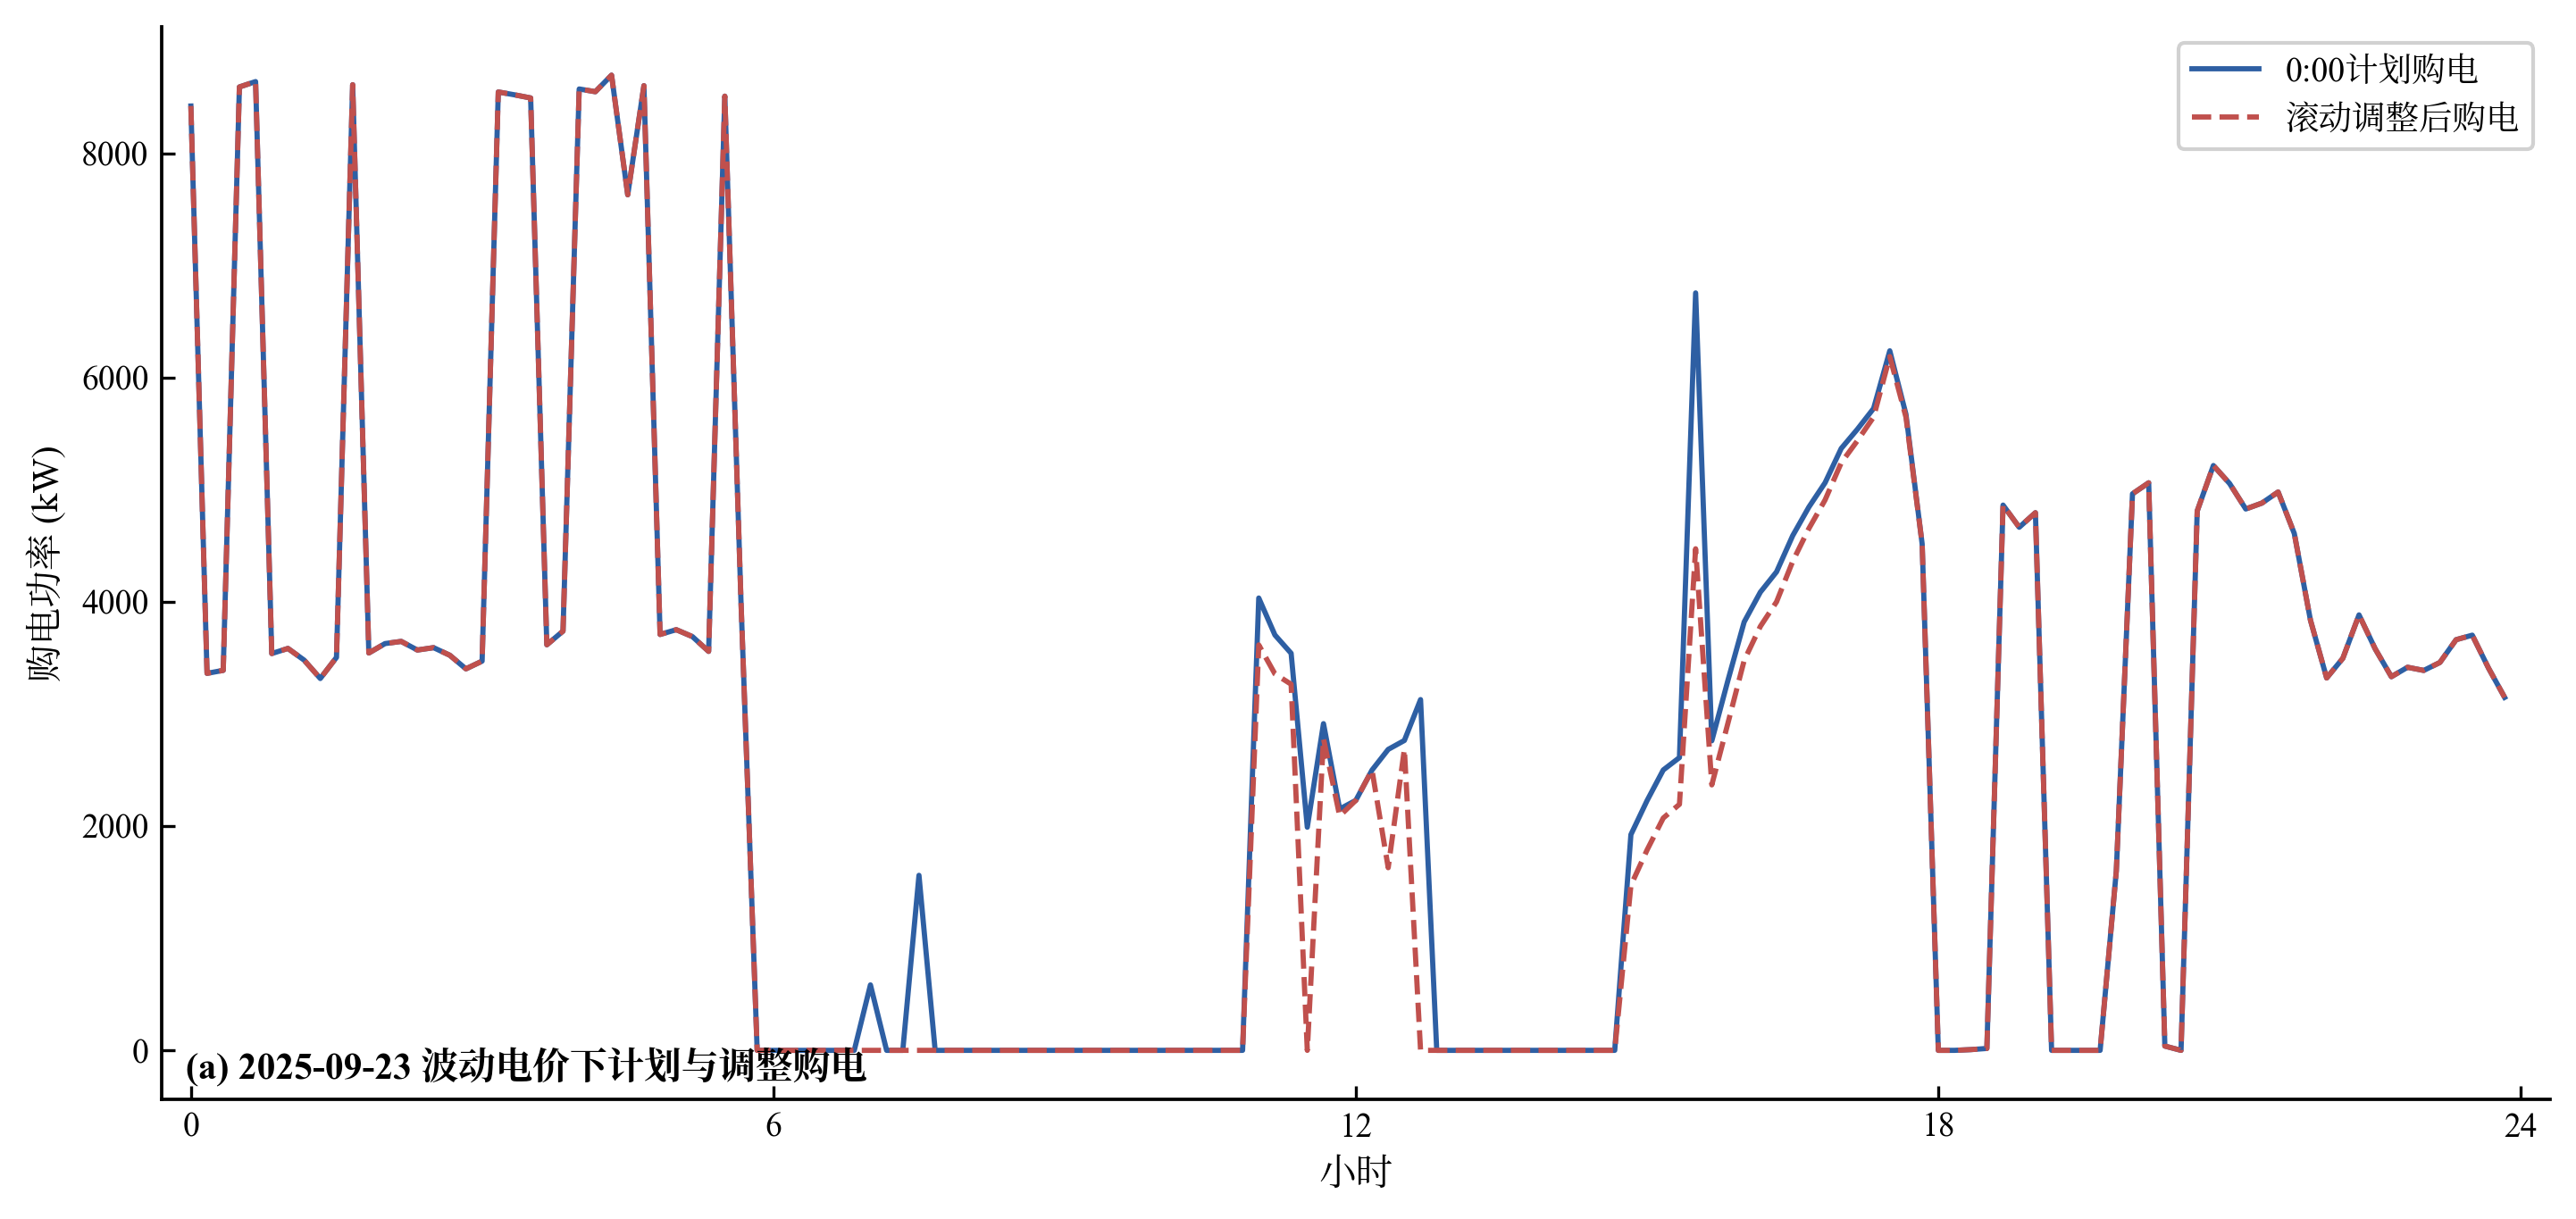
\includegraphics[width=\textwidth]{求解/问题四/图片/图4-3_波动电价滚动调整购电.png}
    \end{minipage}\hfill
    \begin{minipage}[t]{0.44\textwidth}
        \centering
        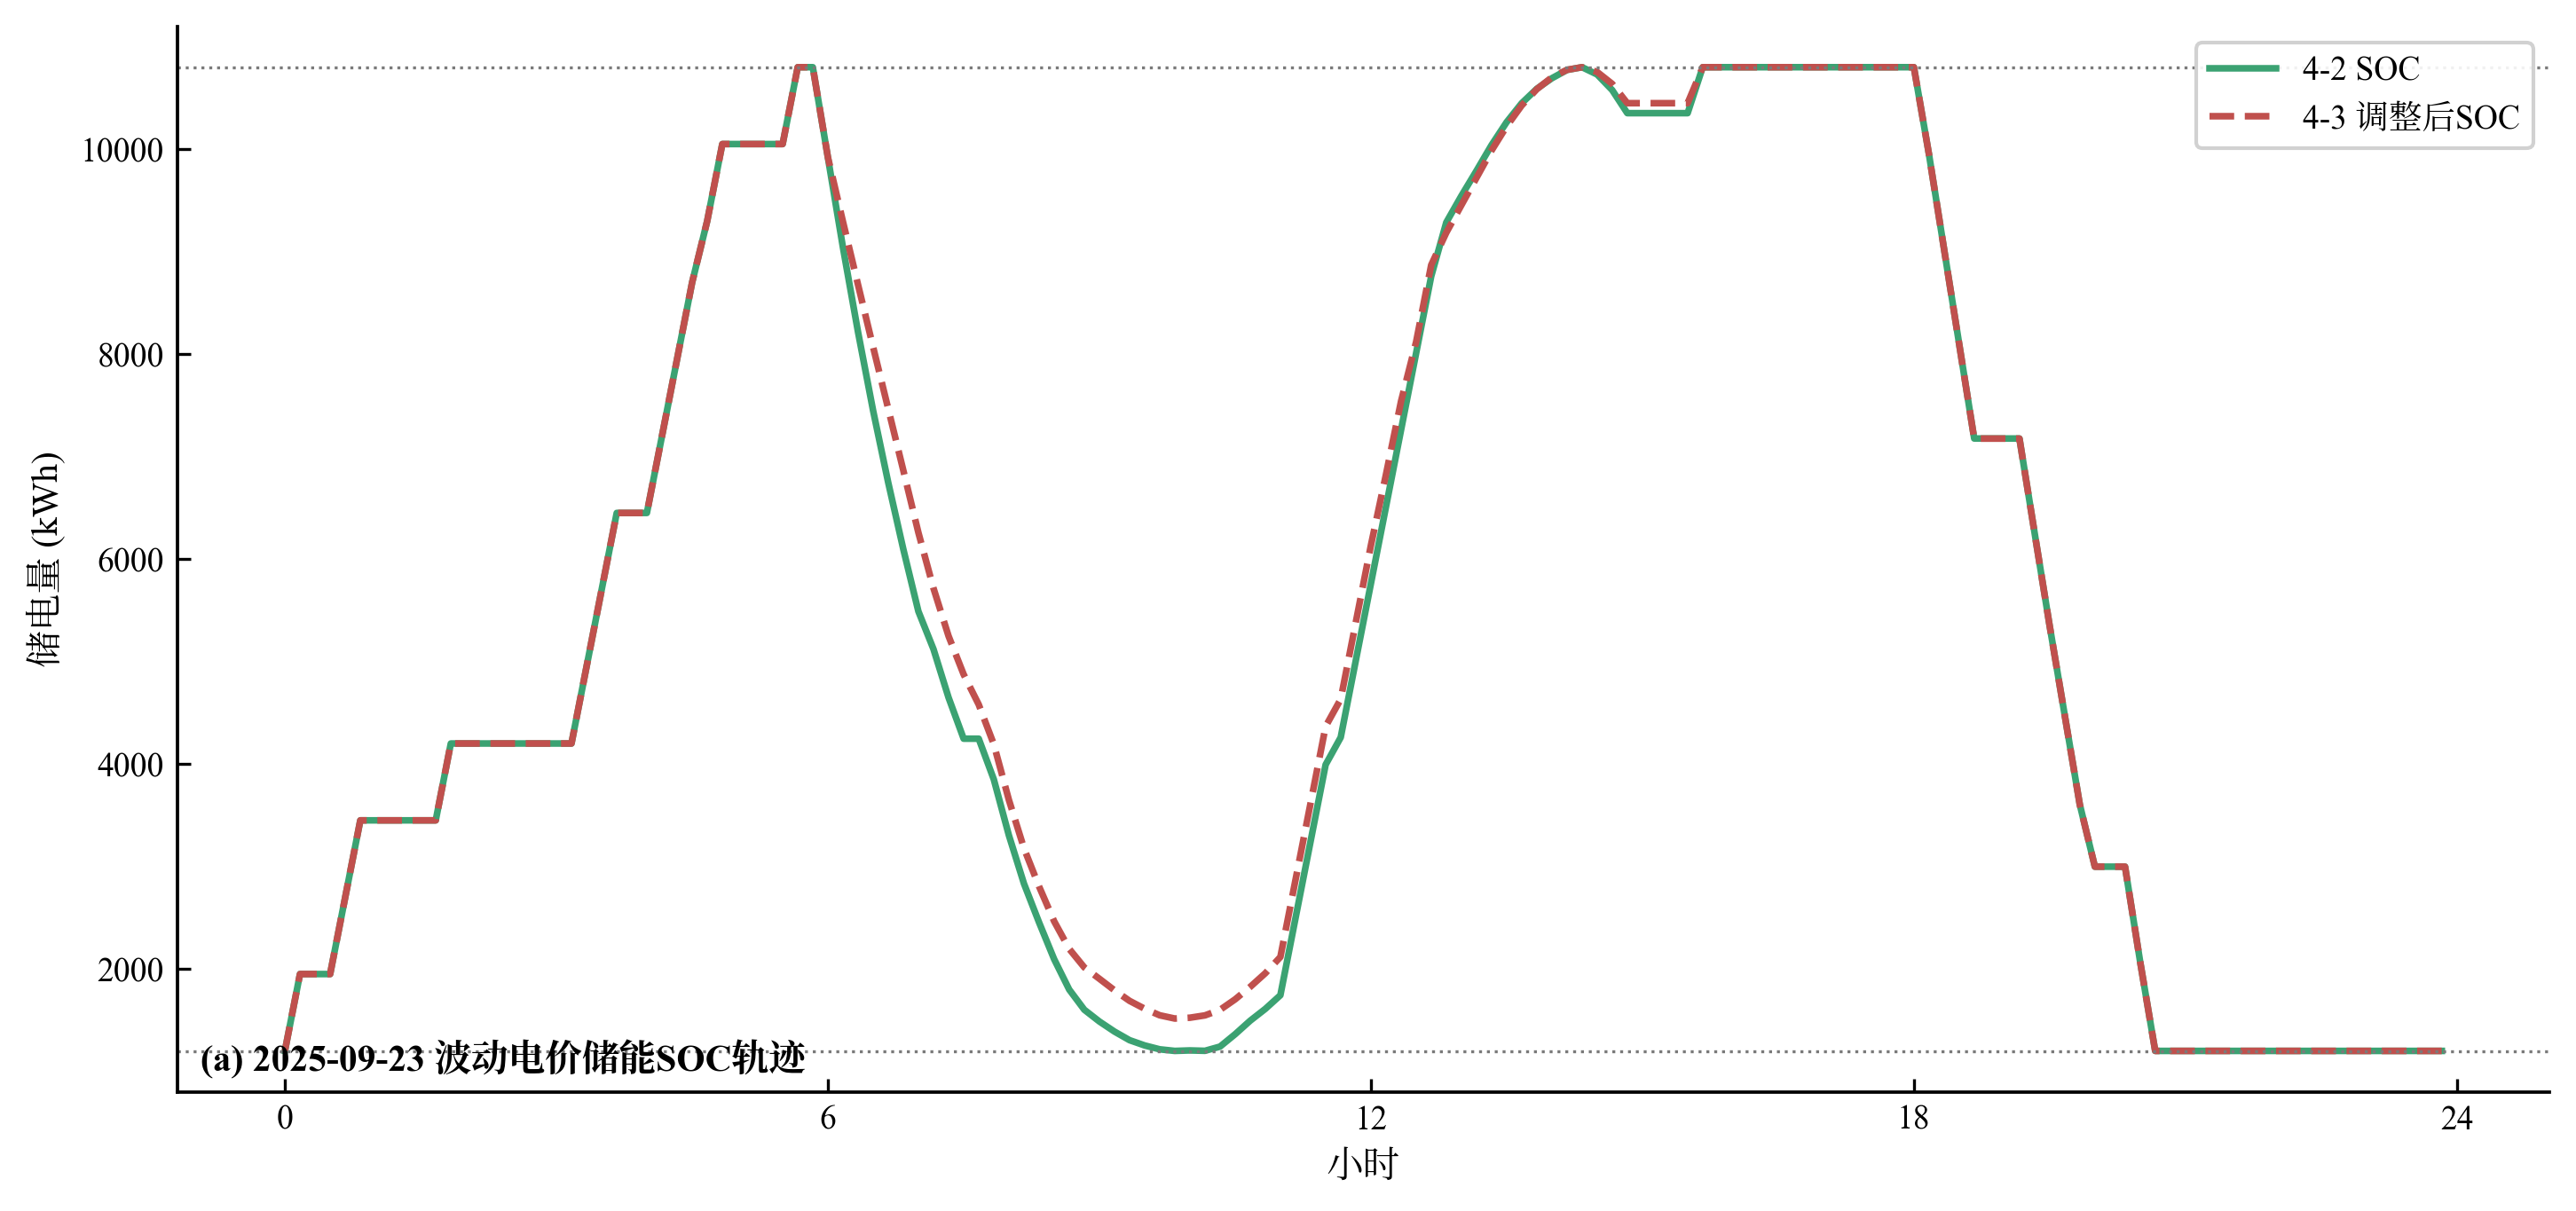
\includegraphics[width=\textwidth]{求解/问题四/图片/图4-4_波动电价SOC轨迹.png}
    \end{minipage}
    \caption{左：波动电价下典型日计划与调整购电对比；右：波动电价下典型日储能荷电状态轨迹}
    \label{fig:结果4-3}
\end{figure}

波动电价下两问费用均高于固定电价情形：问题二由 14382892.99 元升至 15077131.66 元，问题三由 14337999.15 元升至 14956526.18 元，问题三较问题二节省 120605.48 元（约 0.80\%）。费用抬升源于可套利的时段价差被削薄，储能低充高放收益下降，节省率由固定电价时的 3.00\% 降至 0.80\%。本文求解流程不依赖电价的具体形式，沿用固定电价下标定的流程即可得到波动电价下的两套策略。
